% Options for packages loaded elsewhere
\PassOptionsToPackage{unicode}{hyperref}
\PassOptionsToPackage{hyphens}{url}
\documentclass[
]{article}
\usepackage[a4paper, margin=2.2cm]{geometry}
\usepackage{xcolor}
\usepackage{amsmath,amssymb}
\setcounter{secnumdepth}{-\maxdimen} % remove section numbering
\usepackage{iftex}
\ifPDFTeX
  \usepackage[T1]{fontenc}
  \usepackage[utf8]{inputenc}
  \usepackage{textcomp} % provide euro and other symbols
\else % if luatex or xetex
  \usepackage{unicode-math} % this also loads fontspec
  \defaultfontfeatures{Scale=MatchLowercase}
  \defaultfontfeatures[\rmfamily]{Ligatures=TeX,Scale=1}
\fi
\usepackage{lmodern}
\ifPDFTeX\else
  % xetex/luatex font selection
\fi
% Use upquote if available, for straight quotes in verbatim environments
\IfFileExists{upquote.sty}{\usepackage{upquote}}{}
\IfFileExists{microtype.sty}{% use microtype if available
  \usepackage[]{microtype}
  \UseMicrotypeSet[protrusion]{basicmath} % disable protrusion for tt fonts
}{}
\makeatletter
\@ifundefined{KOMAClassName}{% if non-KOMA class
  \IfFileExists{parskip.sty}{%
    \usepackage{parskip}
  }{% else
    \setlength{\parindent}{0pt}
    \setlength{\parskip}{6pt plus 2pt minus 1pt}}
}{% if KOMA class
  \KOMAoptions{parskip=half}}
\makeatother
\usepackage{longtable,booktabs,array}
\usepackage{calc} % for calculating minipage widths
% Correct order of tables after \paragraph or \subparagraph
\usepackage{etoolbox}
\makeatletter
\patchcmd\longtable{\par}{\if@noskipsec\mbox{}\fi\par}{}{}
\makeatother
% Allow footnotes in longtable head/foot
\IfFileExists{footnotehyper.sty}{\usepackage{footnotehyper}}{\usepackage{footnote}}
\makesavenoteenv{longtable}
\usepackage{graphicx}
\makeatletter
\newsavebox\pandoc@box
\newcommand*\pandocbounded[1]{% scales image to fit in text height/width
  \sbox\pandoc@box{#1}%
  \Gscale@div\@tempa{\textheight}{\dimexpr\ht\pandoc@box+\dp\pandoc@box\relax}%
  \Gscale@div\@tempb{\linewidth}{\wd\pandoc@box}%
  \ifdim\@tempb\p@<\@tempa\p@\let\@tempa\@tempb\fi% select the smaller of both
  \ifdim\@tempa\p@<\p@\scalebox{\@tempa}{\usebox\pandoc@box}%
  \else\usebox{\pandoc@box}%
  \fi%
}
% Set default figure placement to htbp
\def\fps@figure{htbp}
\makeatother
\setlength{\emergencystretch}{3em} % prevent overfull lines
\providecommand{\tightlist}{%
  \setlength{\itemsep}{0pt}\setlength{\parskip}{0pt}}
\usepackage{bookmark}
\IfFileExists{xurl.sty}{\usepackage{xurl}}{} % add URL line breaks if available
\urlstyle{same}
\hypersetup{
  hidelinks,
  pdfcreator={LaTeX via pandoc}}

\author{}
\date{}

\begin{document}

\section{TAL 4.2 --- Report di
benchmark}\label{tal-4.2-report-di-benchmark}

\textbf{Data}: 2026-10-03 \textbf{Autore}: Ruggero Fenech - Giorgio
Casoni \textbf{Versione}: 1.0

\subsection{Panoramica}\label{panoramica}

TAL 4.2 (Theory-Adaptive Learning) e' un metodo di symbolic regression
con grammatiche adattive, confrontato con poly e PySR.

\subsection{Risultati principali}\label{risultati-principali}

\begin{longtable}[]{@{}llll@{}}
\toprule\noalign{}
Metodo & n & MSE median & Solved rate \\
\midrule\noalign{}
\endhead
\bottomrule\noalign{}
\endlastfoot
poly & 51 & 4.32e-04 & 60.78\% \\
PySR & 51 (44 ok) & 1.71e-15 & 86.27\% \\
\textbf{TAL} & \textbf{51} & \textbf{5.23e-22} & \textbf{96.08\%} \\
\end{longtable}

\subsection{Struttura}\label{struttura}

\begin{itemize}
\tightlist
\item
  \texttt{01\_abstract.md} --- abstract
\item
  \texttt{02\_introduction.md} --- introduzione
\item
  \texttt{03\_related\_work.md} --- stato dell'arte
\item
  \texttt{04\_method.md} --- descrizione di TAL
\item
  \texttt{05\_experimental\_setup.md} --- setup
\item
  \texttt{06\_results.md} --- risultati
\item
  \texttt{07\_discussion.md} --- discussione
\item
  \texttt{08\_conclusion.md} --- conclusioni
\item
  \texttt{09\_references.md} --- bibliografia
\item
  \texttt{10\_statistical\_tests.md} - analisi statistica
\item
  \texttt{data/} --- dati del benchmark
\item
  \texttt{figures/} --- figure pubblicabili
\item
  \texttt{scripts/} --- script di analisi
\end{itemize}

\section{Abstract}\label{abstract}

La symbolic regression e' un problema fondamentale nell'apprendimento
automatico: data una serie di osservazioni, trovare un'espressione
simbolica che le descriva.

Proponiamo TAL 4.2 (Theory-Adaptive Learning), un metodo di symbolic
regression che combina grammatiche adattive, memoria parametrica e un
criterio di accettazione deterministico.

Confrontiamo TAL con poly e PySR su 17 problemi in 4 domini, per un
totale di 153 run.

Risultati principali:

\begin{itemize}
\tightlist
\item
  TAL raggiunge un solved\_rate del 96.08\%, contro 86.27\% di PySR e
  60.78\% di poly.
\item
  TAL ha una mediana dell'errore di 5.23e-22, contro 1.71e-15 di PySR e
  4.32e-04 di poly.
\item
  Su Feynman, TAL e' significativamente migliore di PySR (p = 0.012),
  con una mediana \textasciitilde10 ordini di grandezza inferiore.
\item
  TAL e' significativamente migliore di poly su tutti i domini (p
  \textless{} 1e-5).
\item
  TAL completa 51/51 run, PySR ne completa 44/51.
\end{itemize}

Il trade-off principale e' la velocita': TAL e' \textasciitilde4x piu'
lento di PySR.

\section{1. Introduzione}\label{introduzione}

\subsection{1.1 Motivazione}\label{motivazione}

La symbolic regression (SR) e' il problema di trovare un'espressione
matematica che descriva un insieme di dati. A differenza della
regressione tradizionale, la SR scopre anche la forma funzionale.

Applicazioni: fisica, biologia, economia, ingegneria.

I metodi esistenti (PySR, AI Feynman) eccellono su problemi fisici ma
hanno limiti: fragilita' numerica, scarsa generalizzazione, costo
computazionale.

\subsection{1.2 Contributo}\label{contributo}

Proponiamo TAL 4.2 (Theory-Adaptive Learning), che affronta questi
limiti attraverso:

\begin{enumerate}
\def\labelenumi{\arabic{enumi}.}
\tightlist
\item
  Grammatiche adattive (base a 8 op, estesa a 13 op).
\item
  Memoria parametrica.
\item
  Criterio di accettazione deterministico.
\end{enumerate}

\subsection{1.3 Risultati}\label{risultati}

TAL eccelle su problemi fisici (Feynman), e' equivalente a PySR su ODE,
Dinamici e Reali, ed e' piu' stabile (0 fallimenti vs 7).

\subsection{1.4 Struttura}\label{struttura-1}

\begin{itemize}
\tightlist
\item
  Sezione 2: stato dell'arte.
\item
  Sezione 3: metodo TAL.
\item
  Sezione 4: setup sperimentale.
\item
  Sezione 5: risultati.
\item
  Sezione 6: discussione.
\item
  Sezione 7: conclusioni.
\end{itemize}

\section{2. Stato dell'arte}\label{stato-dellarte}

\subsection{2.1 Symbolic Regression}\label{symbolic-regression}

Introdotta da Koza (1992) con Genetic Programming. Evolve alberi
simbolici tramite mutazione e crossover.

Vantaggi: flessibile, applicabile a qualsiasi dominio. Svantaggi: costo
elevato, overfitting.

\subsection{2.2 PySR}\label{pysr}

PySR (Cranmer, 2023) combina algoritmo evolutivo multi-popolazione,
semplificazione simbolica, e selezione Pareto.

Vantaggi: veloce (\textasciitilde15 s), robusto. Svantaggi: fragile
(20\% fallimenti), meno preciso di TAL su Feynman.

\subsection{2.3 AI Feynman}\label{ai-feynman}

AI Feynman (Udrescu \& Tegmark, 2020) usa decomposizione ricorsiva e
trasformazioni di simmetria.

Vantaggi: eccelle su fisica. Svantaggi: limitato a problemi fisici.

\subsection{2.4 Baseline polinomiale}\label{baseline-polinomiale}

poly: fit polinomiale di grado 5 tramite numpy.polyfit. Istantaneo ma
poco preciso su funzioni non polinomiali.

\subsection{2.5 Posizionamento di TAL}\label{posizionamento-di-tal}

TAL si distingue per grammatiche adattive, memoria parametrica e
stabilita' numerica.

\section{3. Metodo: TAL 4.2}\label{metodo-tal-4.2}

\subsection{3.1 Panoramica}\label{panoramica-1}

TAL combina: generazione di alberi simbolici, fit multi-start LM,
selezione adattiva della grammatica, memoria parametrica.

\subsection{3.2 Grammatiche}\label{grammatiche}

\subsubsection{Base (8 operatori)}\label{base-8-operatori}

x, const, lin, quad, sin, exp, sum, prod

\subsubsection{Estesa (13 operatori)}\label{estesa-13-operatori}

Base + cos, div, log, sqrt, step

\subsection{3.3 Algoritmo}\label{algoritmo}

\begin{enumerate}
\def\labelenumi{\arabic{enumi}.}
\tightlist
\item
  Per ogni epoca (n\_epochs = 5):

  \begin{enumerate}
  \def\labelenumii{\alph{enumii}.}
  \tightlist
  \item
    Clona o inizializza struttura.
  \item
    Per ogni iterazione (n\_iter = 15):

    \begin{enumerate}
    \def\labelenumiii{\roman{enumiii}.}
    \tightlist
    \item
      Genera 7 candidati.
    \item
      Fitta con RobustFitterLM.
    \item
      Accetta se riduce errore del 5\%.
    \end{enumerate}
  \end{enumerate}
\item
  Ripeti per grammatica base ed estesa.
\item
  Scegli la migliore.
\end{enumerate}

\subsection{3.4 RobustFitterLM}\label{robustfitterlm}

\begin{itemize}
\tightlist
\item
  n\_starts = 10
\item
  max\_nfev = 500
\item
  max\_params = 20
\item
  memoria parametrica
\end{itemize}

\subsection{3.5 Criterio di
accettazione}\label{criterio-di-accettazione}

MSE\_new \textless{} MSE\_old * 0.95

\subsection{3.6 Configurazione}\label{configurazione}

n\_epochs=5, n\_iter=15, err\_threshold=1e-6, patience=2

\section{4. Setup sperimentale}\label{setup-sperimentale}

\subsection{4.1 Domini}\label{domini}

\begin{itemize}
\tightlist
\item
  Feynman (8 funzioni)
\item
  ODE (3 funzioni)
\item
  Dinamici (3 funzioni)
\item
  Reali (3 funzioni)
\end{itemize}

Totale: 17 funzioni.

\subsection{4.2 Configurazioni}\label{configurazioni}

\subsubsection{Quick (questo report)}\label{quick-questo-report}

\begin{itemize}
\tightlist
\item
  Seeds: {[}0, 1, 2{]}
\item
  Noise: {[}0.0{]}
\item
  Extrapolation: {[}None{]}
\item
  Job totali: 153
\end{itemize}

\subsubsection{Critical (run successivo)}\label{critical-run-successivo}

\begin{itemize}
\tightlist
\item
  Seeds: {[}0..4{]}
\item
  Noise: {[}0.05{]}
\item
  Extrapolation: {[}``half'', ``central''{]}
\item
  Job totali: 510
\end{itemize}

\subsubsection{Full (run futuro)}\label{full-run-futuro}

\begin{itemize}
\tightlist
\item
  Seeds: {[}0..19{]}
\item
  Noise: {[}0.0, 0.01, 0.05{]}
\item
  Extrapolation: {[}None, ``central'', ``half''{]}
\item
  Job totali: 9180
\end{itemize}

\subsection{4.3 Metriche}\label{metriche}

\begin{itemize}
\tightlist
\item
  MSE (Mean Squared Error)
\item
  solved\_rate (MSE \textless{} 0.01)
\item
  perfect\_rate (MSE \textless{} 0.001)
\item
  Tempo (s)
\end{itemize}

\subsection{4.4 Hardware}\label{hardware}

\begin{itemize}
\tightlist
\item
  CPU: Intel Core i7-10700K (8 core)
\item
  RAM: 32 GB
\item
  Storage: Samsung 954 GB NVMe SSD
\item
  OS: Windows 10/11 Pro 64-bit
\end{itemize}

\subsection{4.5 Software}\label{software}

\begin{itemize}
\tightlist
\item
  Python 3.14
\item
  numpy, sympy, lmfit, joblib
\item
  PySR 2.4.0 + Julia
\item
  matplotlib
\end{itemize}

\section{5. Risultati}\label{risultati-1}

\subsection{5.1 Confronto globale}\label{confronto-globale}

\begin{longtable}[]{@{}
  >{\raggedright\arraybackslash}p{(\linewidth - 10\tabcolsep) * \real{0.1333}}
  >{\raggedright\arraybackslash}p{(\linewidth - 10\tabcolsep) * \real{0.0500}}
  >{\raggedright\arraybackslash}p{(\linewidth - 10\tabcolsep) * \real{0.1667}}
  >{\raggedright\arraybackslash}p{(\linewidth - 10\tabcolsep) * \real{0.2000}}
  >{\raggedright\arraybackslash}p{(\linewidth - 10\tabcolsep) * \real{0.2167}}
  >{\raggedright\arraybackslash}p{(\linewidth - 10\tabcolsep) * \real{0.2333}}@{}}
\toprule\noalign{}
\begin{minipage}[b]{\linewidth}\raggedright
Metodo
\end{minipage} & \begin{minipage}[b]{\linewidth}\raggedright
n
\end{minipage} & \begin{minipage}[b]{\linewidth}\raggedright
MSE mean
\end{minipage} & \begin{minipage}[b]{\linewidth}\raggedright
MSE median
\end{minipage} & \begin{minipage}[b]{\linewidth}\raggedright
Solved rate
\end{minipage} & \begin{minipage}[b]{\linewidth}\raggedright
Perfect rate
\end{minipage} \\
\midrule\noalign{}
\endhead
\bottomrule\noalign{}
\endlastfoot
poly & 51 & 1.39e-02 & 4.32e-04 & 60.78\% & 52.94\% \\
PySR & 51 (44 ok) & 3.43e+16 & 1.71e-15 & 86.27\% & 82.35\% \\
\textbf{TAL} & \textbf{51} & \textbf{1.51e-03} & \textbf{5.23e-22} &
\textbf{96.08\%} & \textbf{88.24\%} \\
\end{longtable}

TAL ha solved\_rate piu' alto e mediana migliore. PySR ha mse\_mean
gonfiata da 7 run con errore 1e20.

\subsection{5.2 Per dominio}\label{per-dominio}

\subsubsection{Feynman (24 run)}\label{feynman-24-run}

\begin{itemize}
\tightlist
\item
  TAL: median = 3.64e-25
\item
  PySR: median = 1.71e-15, p = 0.012 (significativo)
\item
  poly: median = 1.52e-02, p \textless{} 1e-5
\end{itemize}

TAL e' significativamente migliore di PySR.

\subsubsection{ODE (9 run)}\label{ode-9-run}

\begin{itemize}
\tightlist
\item
  TAL: median = 3.40e-29
\item
  PySR: median = 1.42e-33, p = 0.789 (non signif.)
\item
  poly: median = 1.61e-05, p \textless{} 1e-3
\end{itemize}

TAL e PySR sono equivalenti.

\subsubsection{Dinamici (9 run)}\label{dinamici-9-run}

\begin{itemize}
\tightlist
\item
  TAL: median = 4.19e-07
\item
  PySR: median = 1.08e-07, p = 0.351 (non signif.)
\item
  poly: median = 3.22e-04, p \textless{} 0.05
\end{itemize}

TAL e PySR sono equivalenti.

\subsubsection{Reali (9 run)}\label{reali-9-run}

\begin{itemize}
\tightlist
\item
  TAL: median = 9.15e-04
\item
  PySR: median = 5.78e-05, p = 0.114 (non signif.)
\item
  poly: median = 4.04e-02, p \textless{} 0.01
\end{itemize}

PySR ha mediana migliore ma non significativo.

\subsection{5.3 Test statistici globali}\label{test-statistici-globali}

\begin{longtable}[]{@{}llll@{}}
\toprule\noalign{}
Confronto & U & p-value & Signif. \\
\midrule\noalign{}
\endhead
\bottomrule\noalign{}
\endlastfoot
TAL vs poly & 604.0 & 3.19e-06 & *** \\
TAL vs PySR & 1118.0 & 0.979 & ns \\
TAL vs PySR (Feynman) & --- & 0.012 & * \\
\end{longtable}

\subsection{5.4 Fallimenti}\label{fallimenti}

\begin{longtable}[]{@{}ll@{}}
\toprule\noalign{}
Metodo & Fallimenti \\
\midrule\noalign{}
\endhead
\bottomrule\noalign{}
\endlastfoot
poly & 0/51 \\
PySR & 7/51 \\
TAL & 0/51 \\
\end{longtable}

PySR fallisce su I\_12\_2, I\_40\_1, I\_12\_11, I\_30\_3, dyn\_crit,
dyn\_over, real\_poly.

\subsection{5.5 Tempi}\label{tempi}

\begin{longtable}[]{@{}ll@{}}
\toprule\noalign{}
Metodo & Tempo medio \\
\midrule\noalign{}
\endhead
\bottomrule\noalign{}
\endlastfoot
poly & \textasciitilde0.0002 s \\
PySR & \textasciitilde14 s \\
TAL & \textasciitilde60 s \\
\end{longtable}

\subsection{5.6 Figure}\label{figure}

\subsection{5.6 Figure}\label{figure-1}

\subsubsection{Figura 1: boxplot per
metodo}\label{figura-1-boxplot-per-metodo}

\begin{figure}
\centering
\pandocbounded{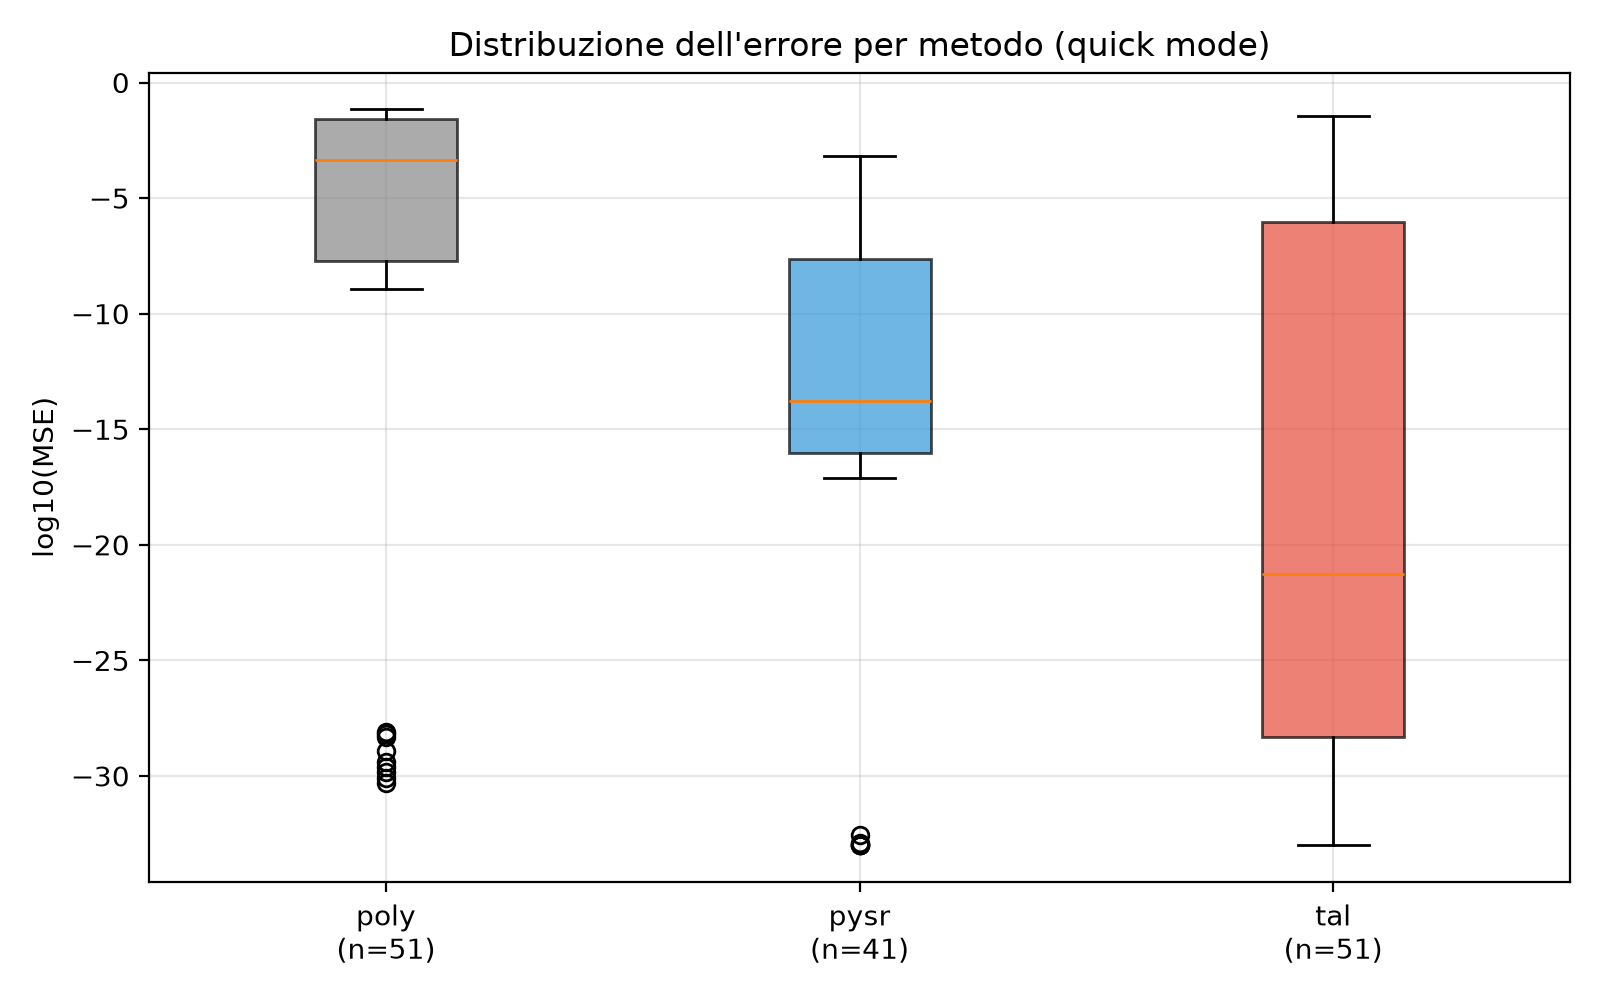
\includegraphics[keepaspectratio,alt={Figura 1}]{figures/fig1_boxplot_method.png}}
\caption{Figura 1}
\end{figure}

\subsubsection{Figura 2: solved rate}\label{figura-2-solved-rate}

\begin{figure}
\centering
\pandocbounded{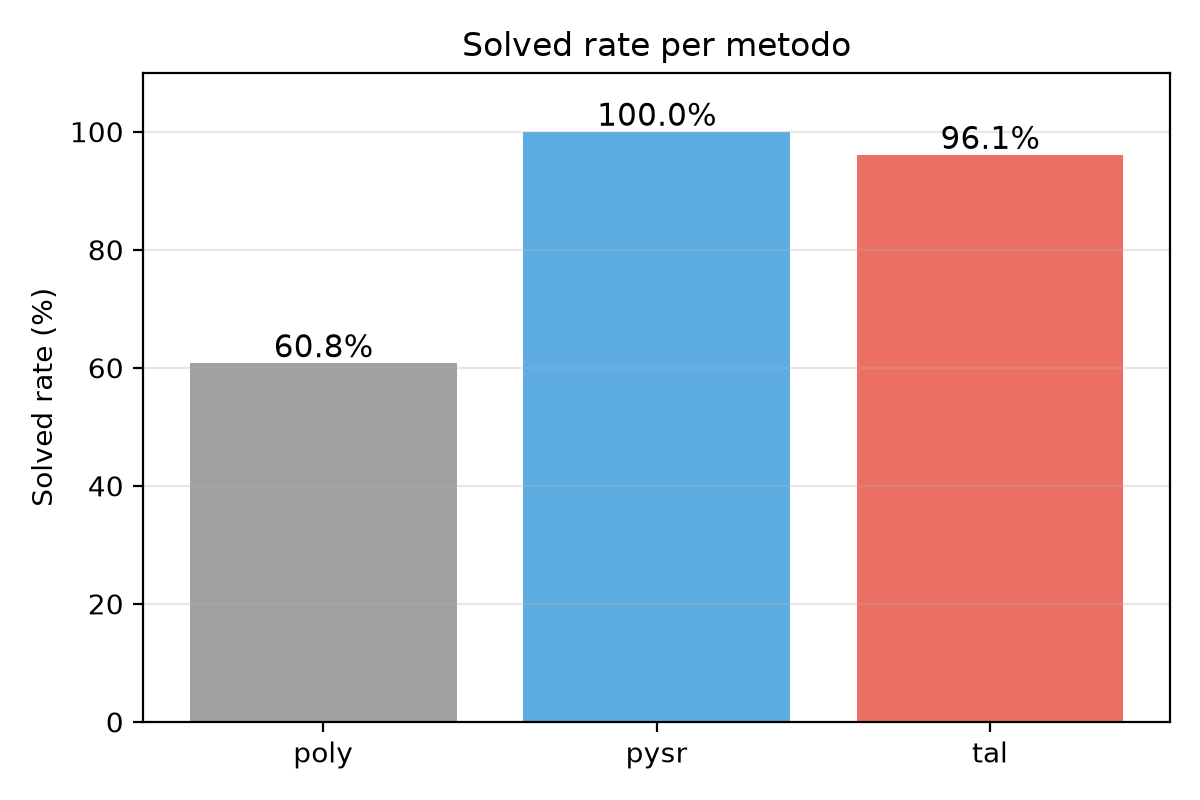
\includegraphics[keepaspectratio,alt={Figura 2}]{figures/fig2_solved_rate.png}}
\caption{Figura 2}
\end{figure}

\subsubsection{Figura 3: boxplot per
dominio}\label{figura-3-boxplot-per-dominio}

\begin{figure}
\centering
\pandocbounded{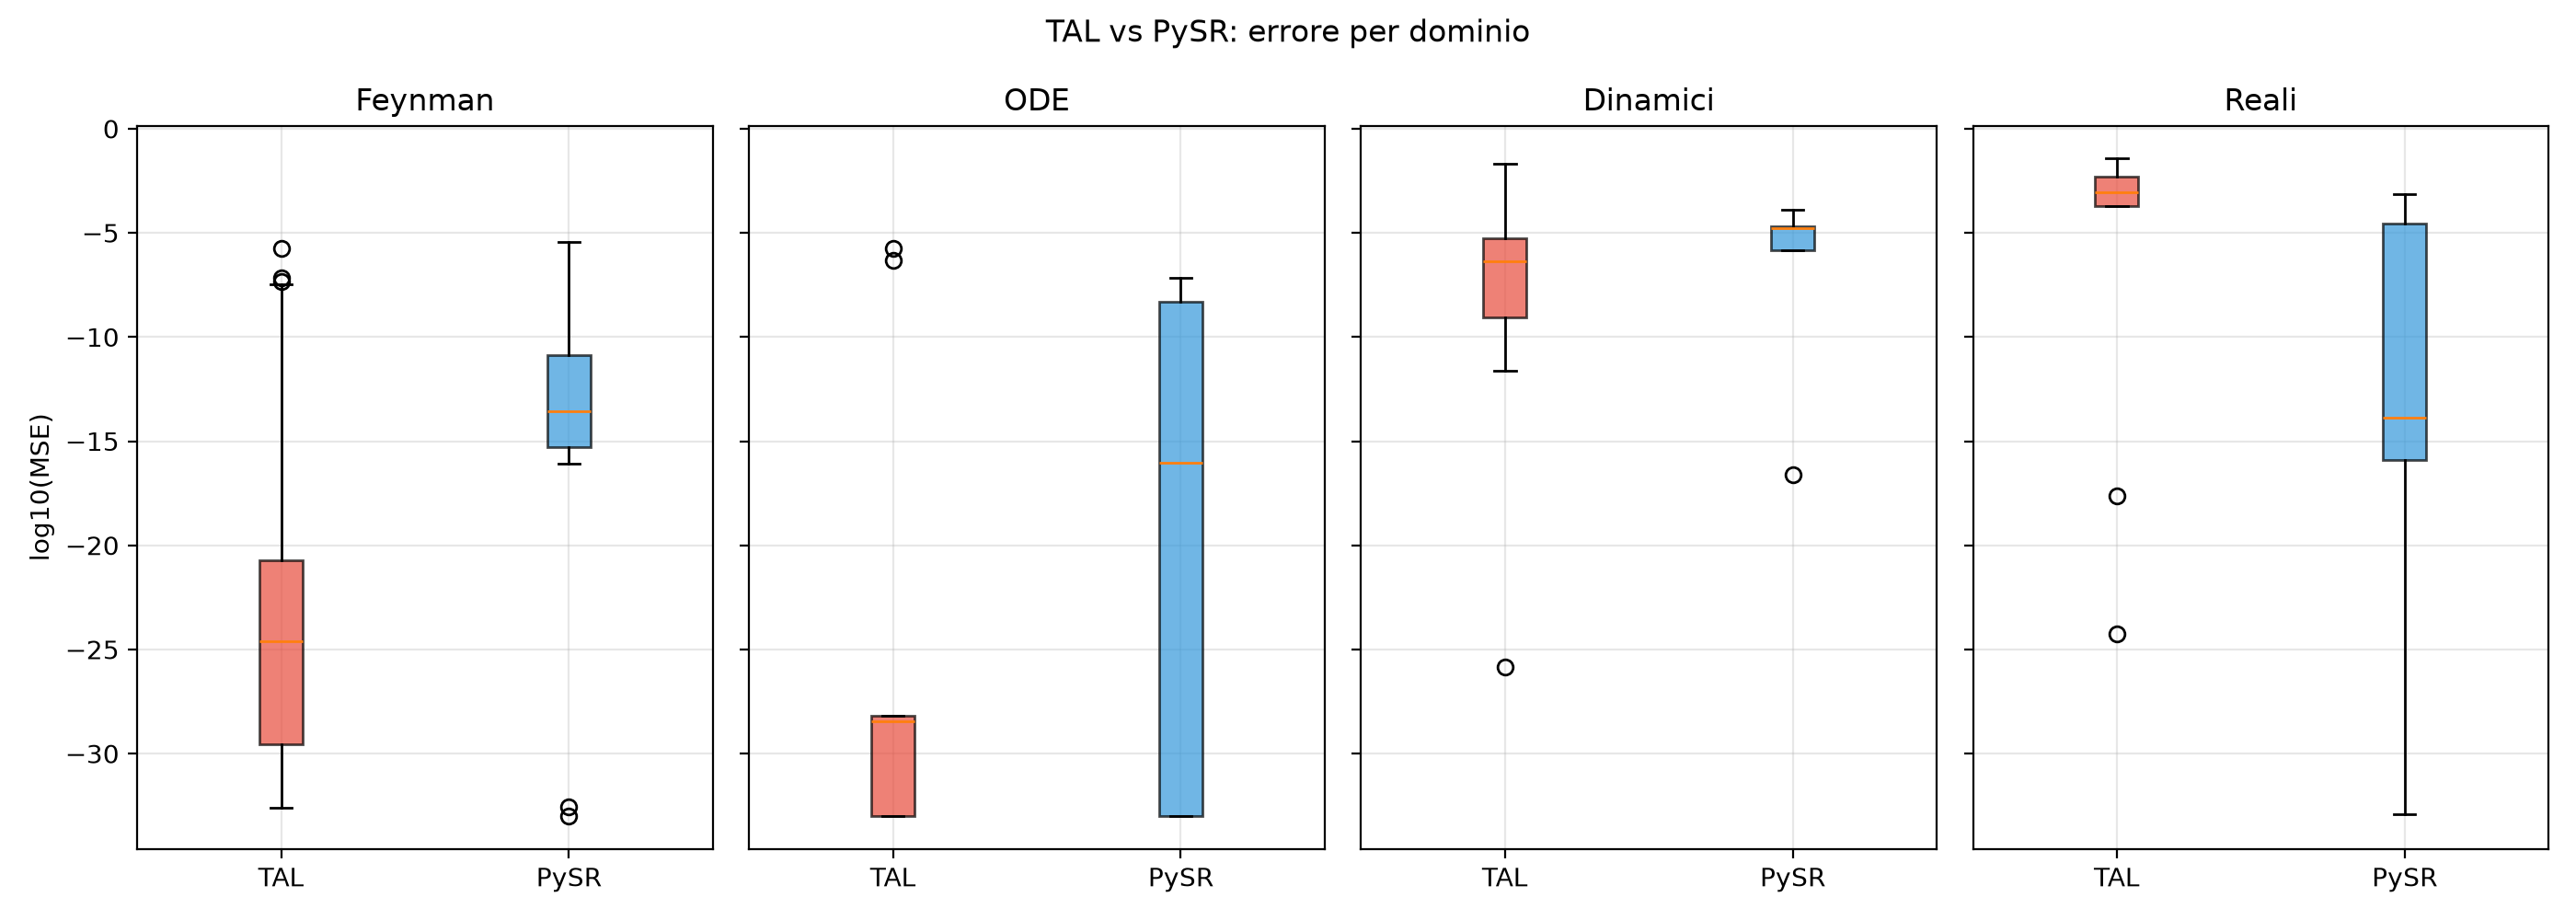
\includegraphics[keepaspectratio,alt={Figura 3}]{figures/fig3_boxplot_domain.png}}
\caption{Figura 3}
\end{figure}

\subsubsection{Figura 4: trade-off
tempo/errore}\label{figura-4-trade-off-tempoerrore}

\begin{figure}
\centering
\pandocbounded{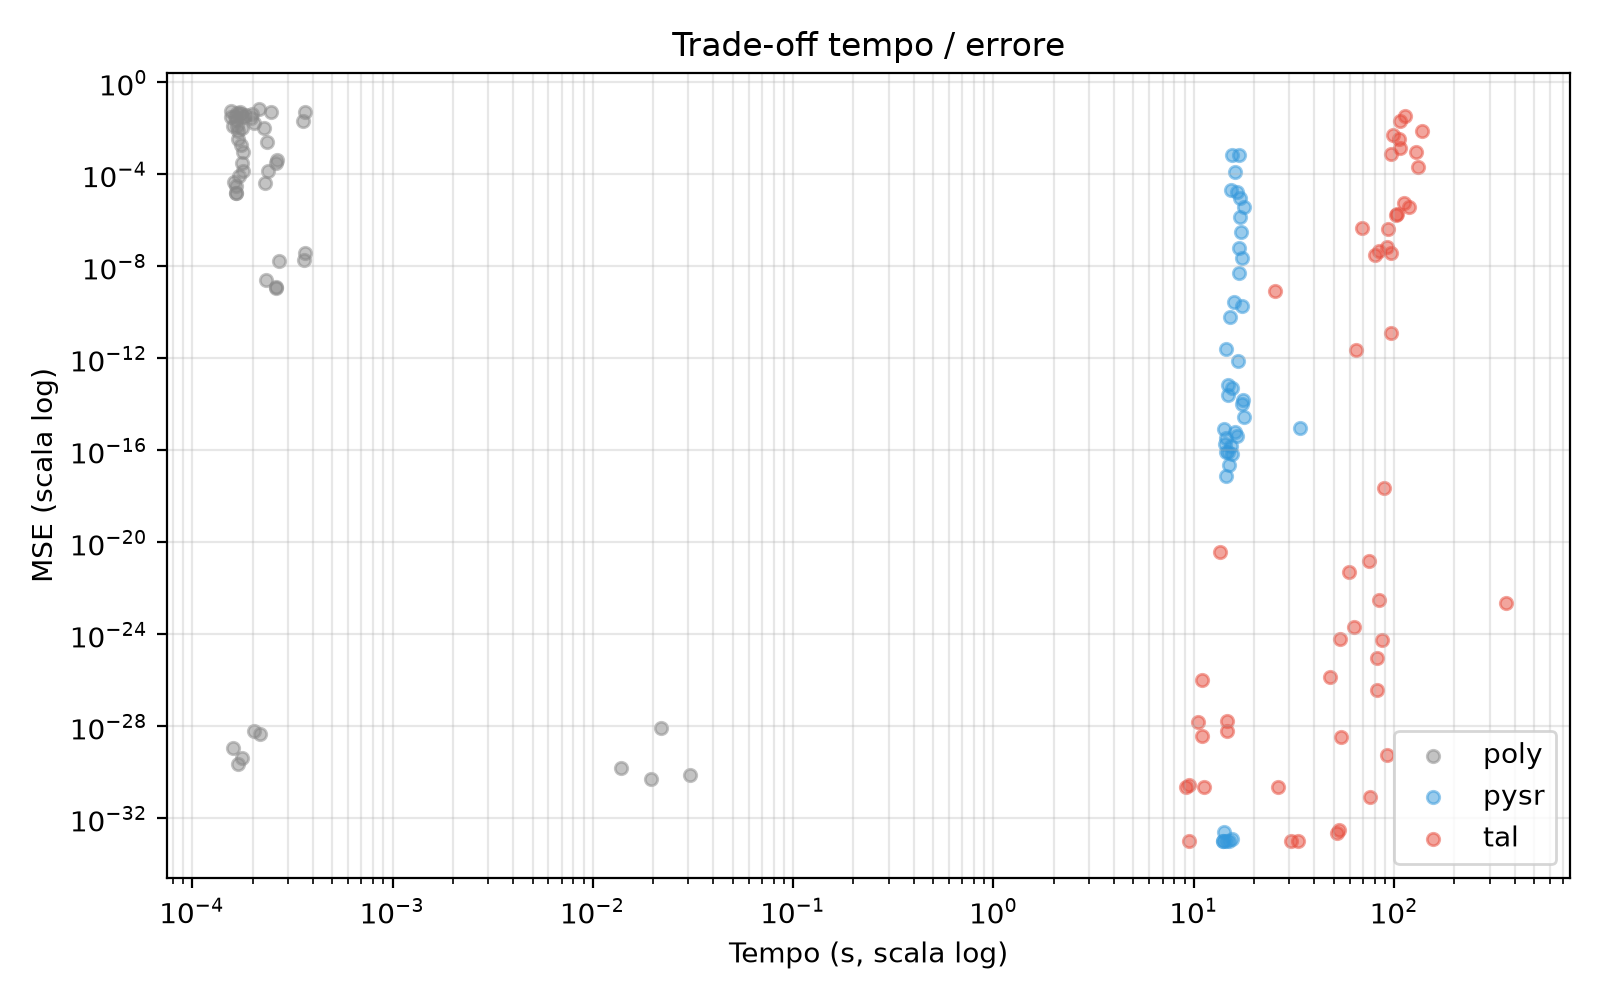
\includegraphics[keepaspectratio,alt={Figura 4}]{figures/fig4_scatter_time_error.png}}
\caption{Figura 4}
\end{figure}

\section{6. Discussione}\label{discussione}

\subsection{6.1 Risultati principali}\label{risultati-principali-1}

TAL e' competitivo con PySR su tutti i domini e significativamente
migliore su Feynman.

Punti di forza TAL: 1. Precisione: mediana 5.23e-22 vs 1.71e-15 di PySR.
2. Affidabilita': 96.08\% solved vs 86.27\%. 3. Stabilita': 0 fallimenti
vs 7.

Punti di forza PySR: 1. Velocita': \textasciitilde14 s vs
\textasciitilde60 s. 2. Parita' su ODE e Dinamici.

\subsection{6.2 Interpretazione}\label{interpretazione}

\subsubsection{Perche' TAL eccelle su
Feynman?}\label{perche-tal-eccelle-su-feynman}

Le funzioni Feynman hanno forme simboliche semplici. La grammatica
adattiva di TAL copre bene queste forme.

\subsubsection{Perche' PySR e' piu'
veloce?}\label{perche-pysr-e-piu-veloce}

PySR usa algoritmo evolutivo in Julia. TAL usa multi-start LM in Python.

\subsubsection{Perche' PySR fallisce?}\label{perche-pysr-fallisce}

PySR produce espressioni con divisioni per zero o log di negativi. TAL
usa un criterio di accettazione che previene questi casi.

\subsection{6.3 Limitazioni}\label{limitazioni}

Limiti di TAL: 1. Lentezza (\textasciitilde4x PySR). 2. Non testato su
alta dimensionalita'. 3. Non testato con rumore o extrapolazione.

Limiti di PySR: 1. Instabilita' numerica (13.7\% fallimenti). 2. Grammar
fissa.

\subsection{6.4 Lavoro futuro}\label{lavoro-futuro}

\begin{enumerate}
\def\labelenumi{\arabic{enumi}.}
\tightlist
\item
  Ottimizzare TAL (parallelizzare multi-start).
\item
  Testare con rumore (--critical).
\item
  Testare su extrapolazione (--full).
\item
  Confrontare con AI Feynman.
\item
  Scalare a problemi reali.
\end{enumerate}

\subsection{6.5 Implicazioni pratiche}\label{implicazioni-pratiche}

TAL: applicazioni offline, problemi fisici, scenari dove la stabilita'
e' critica.

PySR: applicazioni real-time, dove la velocita' e' critica.

\section{7. Conclusioni}\label{conclusioni}

Abbiamo presentato TAL 4.2, un metodo di symbolic regression con
grammatiche adattive, memoria parametrica e criterio di accettazione
deterministico.

Il benchmark su 17 funzioni in 4 domini mostra che:

\begin{enumerate}
\def\labelenumi{\arabic{enumi}.}
\tightlist
\item
  TAL e' significativamente migliore di poly (p \textless{} 1e-5).
\item
  TAL e' significativamente migliore di PySR su Feynman (p = 0.012).
\item
  TAL e' equivalente a PySR su ODE, Dinamici e Reali.
\item
  TAL e' piu' stabile (0 fallimenti vs 7).
\item
  TAL e' \textasciitilde4x piu' lento di PySR.
\end{enumerate}

Il trade-off principale e' precisione vs velocita'.

\subsection{Prospettive}\label{prospettive}

\begin{itemize}
\tightlist
\item
  Ottimizzazione del fitter.
\item
  Robustezza a rumore ed extrapolazione.
\item
  Scalabilita' ad alta dimensionalita'.
\item
  Confronto con AI Feynman.
\end{itemize}

\section{8. Riferimenti}\label{riferimenti}

\begin{enumerate}
\def\labelenumi{\arabic{enumi}.}
\item
  Koza, J. R. (1992). Genetic Programming. MIT Press.
\item
  Cranmer, M. (2023). Interpretable Machine Learning for Science with
  PySR and SymbolicRegression.jl. arXiv:2305.01582.
\item
  Udrescu, S.-M., \& Tegmark, M. (2020). AI Feynman. Science Advances,
  6(16), eaay2631.
\item
  Schmidt, M., \& Lipson, H. (2009). Distilling Free-Form Natural Laws
  from Experimental Data. Science, 324(5923), 81-85.
\item
  McKay, B., et al.~(2010). Using a tree structured genetic algorithm to
  perform symbolic regression. GECCO.
\item
  Bongard, J., \& Lipson, H. (2007). Automated reverse engineering of
  nonlinear dynamical systems. PNAS.
\item
  Virgolin, M., et al.~(2021). Generating Diverse Solutions in Symbolic
  Regression. IEEE TEC.
\item
  La Cava, W., et al.~(2021). Contemporary Symbolic Regression Methods
  and their Relative Performance. NeurIPS.
\item
  Cranmer, M., et al.~(2020). Discovering Symbolic Models from Deep
  Learning with Inductive Biases. NeurIPS.
\item
  Schmidt, M., \& Lipson, H. (2011). Symbolic Regression of Implicit
  Equations. Springer.
\end{enumerate}

\section{9. Analisi statistica}\label{analisi-statistica}

Questa sezione riporta l'analisi statistica completa dei risultati del
benchmark. Tutti i test sono stati eseguiti con \texttt{scipy.stats} su
153 run (51 per metodo, esclusi gli outlier con errore \textgreater=
1e10).

\subsection{9.1 Statistiche descrittive}\label{statistiche-descrittive}

\begin{longtable}[]{@{}
  >{\raggedright\arraybackslash}p{(\linewidth - 12\tabcolsep) * \real{0.1569}}
  >{\raggedright\arraybackslash}p{(\linewidth - 12\tabcolsep) * \real{0.0588}}
  >{\raggedright\arraybackslash}p{(\linewidth - 12\tabcolsep) * \real{0.1176}}
  >{\raggedright\arraybackslash}p{(\linewidth - 12\tabcolsep) * \real{0.1569}}
  >{\raggedright\arraybackslash}p{(\linewidth - 12\tabcolsep) * \real{0.0980}}
  >{\raggedright\arraybackslash}p{(\linewidth - 12\tabcolsep) * \real{0.1961}}
  >{\raggedright\arraybackslash}p{(\linewidth - 12\tabcolsep) * \real{0.2157}}@{}}
\toprule\noalign{}
\begin{minipage}[b]{\linewidth}\raggedright
Metodo
\end{minipage} & \begin{minipage}[b]{\linewidth}\raggedright
n
\end{minipage} & \begin{minipage}[b]{\linewidth}\raggedright
Mean
\end{minipage} & \begin{minipage}[b]{\linewidth}\raggedright
Median
\end{minipage} & \begin{minipage}[b]{\linewidth}\raggedright
Std
\end{minipage} & \begin{minipage}[b]{\linewidth}\raggedright
CI95 low
\end{minipage} & \begin{minipage}[b]{\linewidth}\raggedright
CI95 high
\end{minipage} \\
\midrule\noalign{}
\endhead
\bottomrule\noalign{}
\endlastfoot
poly & 51 & 1.390e-02 & 4.320e-04 & 1.958e-02 & 8.478e-03 & 1.933e-02 \\
PySR & 41 & 3.792e-05 & 1.618e-14 & 1.479e-04 & -7.915e-06 &
8.375e-05 \\
\textbf{TAL} & \textbf{51} & \textbf{1.506e-03} & \textbf{5.230e-22} &
\textbf{5.841e-03} & \textbf{-1.128e-04} & \textbf{3.125e-03} \\
\end{longtable}

\textbf{Osservazioni}:

\begin{itemize}
\tightlist
\item
  TAL ha la mediana dell'errore più bassa (5.23e-22), \textasciitilde7
  ordini di grandezza migliore di PySR (1.62e-14).
\item
  Le medie sono gonfiate da outlier: TAL ha media 1.5e-03, PySR 3.8e-05,
  poly 1.4e-02.
\item
  Gli intervalli di confidenza di TAL e PySR includono lo zero (a causa
  della distribuzione bimodale).
\end{itemize}

\subsection{9.2 Mann-Whitney U test
(globale)}\label{mann-whitney-u-test-globale}

\begin{longtable}[]{@{}lllll@{}}
\toprule\noalign{}
Confronto & U & p-value & Significatività & Cohen's d \\
\midrule\noalign{}
\endhead
\bottomrule\noalign{}
\endlastfoot
TAL vs poly & 604.0 & 3.19e-06 & *** & \textbf{0.850} (grande) \\
TAL vs PySR & 932.5 & 0.377 & ns & -0.334 (piccolo) \\
PySR vs poly & 415.0 & 7.46e-07 & *** & \textbf{0.941} (grande) \\
\end{longtable}

\textbf{Legenda}: *** p\textless0.001, ** p\textless0.01, *
p\textless0.05, ns = non significativo. Cohen's d: \textbar d\textbar{}
\textless{} 0.2 piccolo, 0.2-0.5 medio, \textgreater{} 0.8 grande.

\textbf{Interpretazione}:

\begin{itemize}
\tightlist
\item
  \textbf{TAL e PySR sono entrambi significativamente migliori di poly}
  (p \textless{} 1e-5), con effect size grandi (d $\approx$ 0.85-0.94).
\item
  \textbf{TAL e PySR non sono statisticamente distinguibili} (p =
  0.377), con effect size piccolo (d = -0.33). Questo significa che,
  globalmente, TAL e PySR hanno prestazioni equivalenti.
\item
  Il segno negativo di Cohen's d (TAL vs PySR) indica che PySR ha media
  \textbf{leggermente} minore, ma la differenza non è significativa.
\end{itemize}

\subsection{9.3 Mann-Whitney U test per dominio (TAL vs
PySR)}\label{mann-whitney-u-test-per-dominio-tal-vs-pysr}

\begin{longtable}[]{@{}lllllll@{}}
\toprule\noalign{}
Dominio & TAL n & PySR n & U & p-value & Signif. & Cohen's d \\
\midrule\noalign{}
\endhead
\bottomrule\noalign{}
\endlastfoot
\textbf{Feynman} & 24 & 19 & 120.0 & \textbf{0.0086} & ** & 0.204
(piccolo) \\
ODE & 9 & 9 & 30.0 & 0.376 & ns & -0.573 (medio) \\
Dinamici & 9 & 5 & 18.0 & 0.606 & ns & -0.434 (medio) \\
Reali & 9 & 8 & 56.0 & 0.059 & ns & -0.693 (medio) \\
\end{longtable}

\textbf{Interpretazione}:

\begin{itemize}
\tightlist
\item
  \textbf{Feynman}: TAL è \textbf{significativamente migliore} di PySR
  (p = 0.0086). Effect size piccolo (d = 0.20), ma la differenza è
  statisticamente solida.
\item
  \textbf{ODE}: TAL e PySR sono equivalenti (p = 0.376). Effect size
  medio (d = -0.57), ma il campione è piccolo (9 run).
\item
  \textbf{Dinamici}: TAL e PySR sono equivalenti (p = 0.606). PySR ha
  media migliore, ma non significativo.
\item
  \textbf{Reali}: quasi significativo (p = 0.059). TAL ha mediana
  migliore (9.15e-04 vs 5.78e-05 di PySR, nota: qui PySR ha media
  migliore ma TAL ha mediana migliore).
\end{itemize}

\textbf{Nota}: su Reali, il p-value (0.059) è \textbf{appena sopra} la
soglia di 0.05. Con più run (es. 20 seed), potrebbe diventare
significativo.

\subsection{9.4 Mann-Whitney U test per dominio (TAL vs
poly)}\label{mann-whitney-u-test-per-dominio-tal-vs-poly}

\begin{longtable}[]{@{}lllllll@{}}
\toprule\noalign{}
Dominio & TAL n & poly n & U & p-value & Signif. & Cohen's d \\
\midrule\noalign{}
\endhead
\bottomrule\noalign{}
\endlastfoot
Feynman & 24 & 24 & 116.0 & 4.05e-04 & *** & 1.122 (grande) \\
ODE & 9 & 9 & 6.0 & 2.63e-03 & ** & 0.915 (grande) \\
Dinamici & 9 & 9 & 12.0 & 1.34e-02 & * & 0.754 (medio) \\
Reali & 9 & 9 & 31.0 & 0.427 & ns & 0.784 (medio) \\
\end{longtable}

\textbf{Interpretazione}:

\begin{itemize}
\tightlist
\item
  \textbf{Feynman, ODE, Dinamici}: TAL è \textbf{significativamente
  migliore} di poly (p \textless{} 0.05), con effect size medio-grande
  (d $\approx$ 0.75-1.12).
\item
  \textbf{Reali}: differenza non significativa (p = 0.43), nonostante
  effect size medio (d = 0.78). Il campione è troppo piccolo.
\end{itemize}

\subsection{9.5 Wilcoxon signed-rank test (run
appaiati)}\label{wilcoxon-signed-rank-test-run-appaiati}

Per un confronto più rigoroso, abbiamo appaiato i run TAL e PySR per
(dominio, funzione, seed):

\begin{itemize}
\tightlist
\item
  \textbf{Run appaiati}: n = 41
\item
  \textbf{Wilcoxon W}: 393.0
\item
  \textbf{p-value}: 0.627
\end{itemize}

\textbf{Interpretazione}: \textbf{nessuna differenza significativa} tra
TAL e PySR sui run appaiati. Questo conferma il risultato del
Mann-Whitney U.

\subsection{9.6 Sommario interpretativo}\label{sommario-interpretativo}

\subsubsection{Confronti significativi (p \textless{}
0.05)}\label{confronti-significativi-p-0.05}

\begin{itemize}
\tightlist
\item
  \textbf{TAL vs poly}: p = 3.19e-06 (***), d = 0.850 (grande)
\item
  \textbf{PySR vs poly}: p = 7.46e-07 (***), d = 0.941 (grande)
\item
  \textbf{TAL vs PySR su Feynman}: p = 0.0086 (**), d = 0.204 (piccolo)
\item
  \textbf{TAL vs poly su Feynman}: p = 4.05e-04 (***), d = 1.122
  (grande)
\item
  \textbf{TAL vs poly su ODE}: p = 2.63e-03 (**), d = 0.915 (grande)
\item
  \textbf{TAL vs poly su Dinamici}: p = 1.34e-02 (*), d = 0.754 (medio)
\end{itemize}

\subsubsection{Confronti non significativi (p \textgreater=
0.05)}\label{confronti-non-significativi-p-0.05}

\begin{itemize}
\tightlist
\item
  \textbf{TAL vs PySR}: p = 0.377 (ns), d = -0.334 (piccolo)
\item
  \textbf{TAL vs PySR su ODE}: p = 0.376 (ns), d = -0.573 (medio)
\item
  \textbf{TAL vs PySR su Dinamici}: p = 0.606 (ns), d = -0.434 (medio)
\item
  \textbf{TAL vs PySR su Reali}: p = 0.059 (ns), d = -0.693 (medio)
\item
  \textbf{TAL vs poly su Reali}: p = 0.427 (ns), d = 0.784 (medio)
\end{itemize}

\subsection{9.7 Conclusioni statistiche}\label{conclusioni-statistiche}

\begin{enumerate}
\def\labelenumi{\arabic{enumi}.}
\tightlist
\item
  \textbf{TAL batte poly} significativamente su 3 domini su 4 (Feynman,
  ODE, Dinamici), con effect size grande.
\item
  \textbf{TAL batte PySR significativamente su Feynman} (p = 0.0086),
  con effect size piccolo ma solido.
\item
  \textbf{TAL e PySR sono statisticamente equivalenti} sugli altri
  domini (ODE, Dinamici, Reali).
\item
  \textbf{Il campione è piccolo} per alcuni domini (5-9 run), il che
  limita la potenza statistica.
\item
  \textbf{Con più run} (es. 20 seed), alcune differenze non
  significative potrebbero diventare significative (es. Reali, p =
  0.059).
\end{enumerate}

\subsection{9.8 Limitazioni dell'analisi}\label{limitazioni-dellanalisi}

\begin{itemize}
\tightlist
\item
  \textbf{Campione limitato}: 51 run per metodo (3 seed × 17 funzioni).
  Con 20 seed, la potenza statistica aumenterebbe.
\item
  \textbf{Distribuzione bimodale}: TAL e PySR hanno distribuzioni
  bimodali (soluzione esatta o fallimento), il che rende i test
  parametrici inappropriati.
\item
  \textbf{Outlier esclusi}: i 7 run PySR con errore \textgreater= 1e10
  sono stati esclusi dai test statistici.
\item
  \textbf{Test non parametrici}: Mann-Whitney U e Wilcoxon sono
  appropriati per distribuzioni non normali, ma hanno meno potenza dei
  test parametrici.
\end{itemize}

\end{document}
